\documentclass[11pt,letterpaper,twoside]{article}
\usepackage[english]{babel}
\usepackage{amssymb,amsmath}
\usepackage{fancyhdr}
\usepackage{graphicx}

 \oddsidemargin  0in \evensidemargin 0in
 \topmargin   -0.25in \headheight 0.25in \headsep 0.25in
 \textwidth   6.5in \textheight 8.75in \marginparsep 0pt \marginparwidth 0pt
 \parskip 1ex  \parindent 0ex \footskip 20pt

\newfont{\bssten}{cmssbx10}
\newfont{\bssnine}{cmssbx10 scaled 900}

%%%%%%%%%%%%%%%%%%%%%%%
\newcommand{\whatizit}{Lecture 7: Correlation}
%%%%%%%%%%%%%%%%%%%%%%%


\pagestyle{fancy}  
\fancyhead{\bssnine STOR 155,  \whatizit}
\fancyhead[RE]{} \fancyhead[LO]{}
\fancyhead[LE]{\bssnine \thepage} \fancyhead[RO]{\bssnine \thepage}
\lfoot{} \cfoot{} \rfoot{}   


\newcommand{\var}{\mathrm{Var}}



\begin{document}



\thispagestyle{empty} \vspace*{-0.75in}

{\bssten STOR 155: Introduction to Data Models and Inference \hfill May 21, 2024 \\
Prof. Will Lassiter  \hfill Page 1 of \pageref{totalpag}}
\vspace{10pt}
\begin{center} {{\Large \bf \whatizit}} \end{center}

{\bf Using Correlation to Measure Strength of Association} \vspace{6pt}

Which scatter plot below displays a stronger linear association?

\begin{center}

\includegraphics[scale=0.8]{images/scatters.png}
\end{center}

{\bf Correlation}, which we will denote with $r$, gives us a more mathematical way to measure the strength of the linear association between two numerical variables: $$r=\frac{1}{n-1}\sum_{i=1}^n \left(\frac{x_i-\bar{x}}{s_x}\right)\left(\frac{y_i-\bar{y}}{s_y}\right) $$

\vspace{100pt}

Practice: Find correlation between $X$ and $Y$ given the observations below:

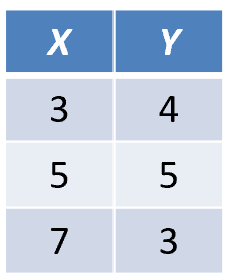
\includegraphics[scale=0.8]{images/obs.png}

\newpage

{\bf Properties of Correlation}

\begin{itemize}

\item Possible values \vspace{50pt}

\item Sign meaning \vspace{50pt}

\item $r$ does not change even if we... \vspace{50pt}

\item Note on outliers \vspace{30pt}

\end{itemize}

Examples: 

\begin{center}

\includegraphics[scale=0.8]{images/scatters2.png}
\end{center}

$$r=\frac{1}{n-1}\sum_{i=1}^n \left(\frac{x_i-\bar{x}}{s_x}\right)\left(\frac{y_i-\bar{y}}{s_y}\right) $$

\newpage

How an outlier can distort an association:

\begin{center}
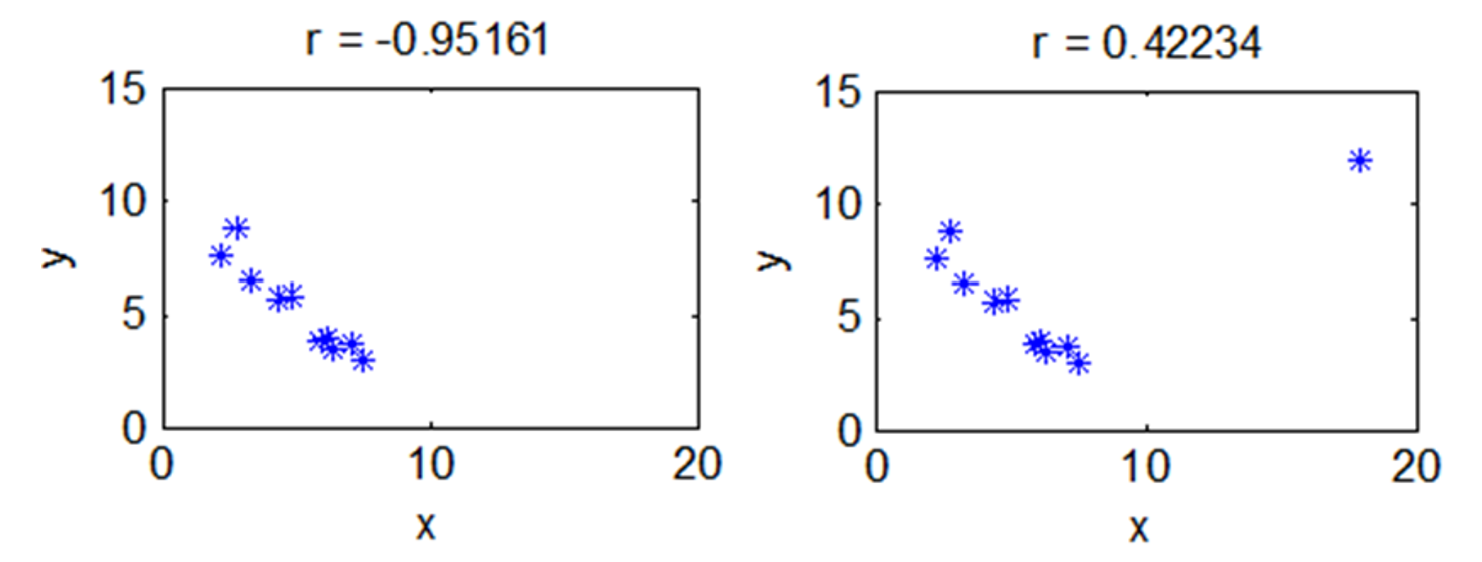
\includegraphics[scale=0.6]{images/outlier.png}
\end{center}

Another example:

\begin{center}
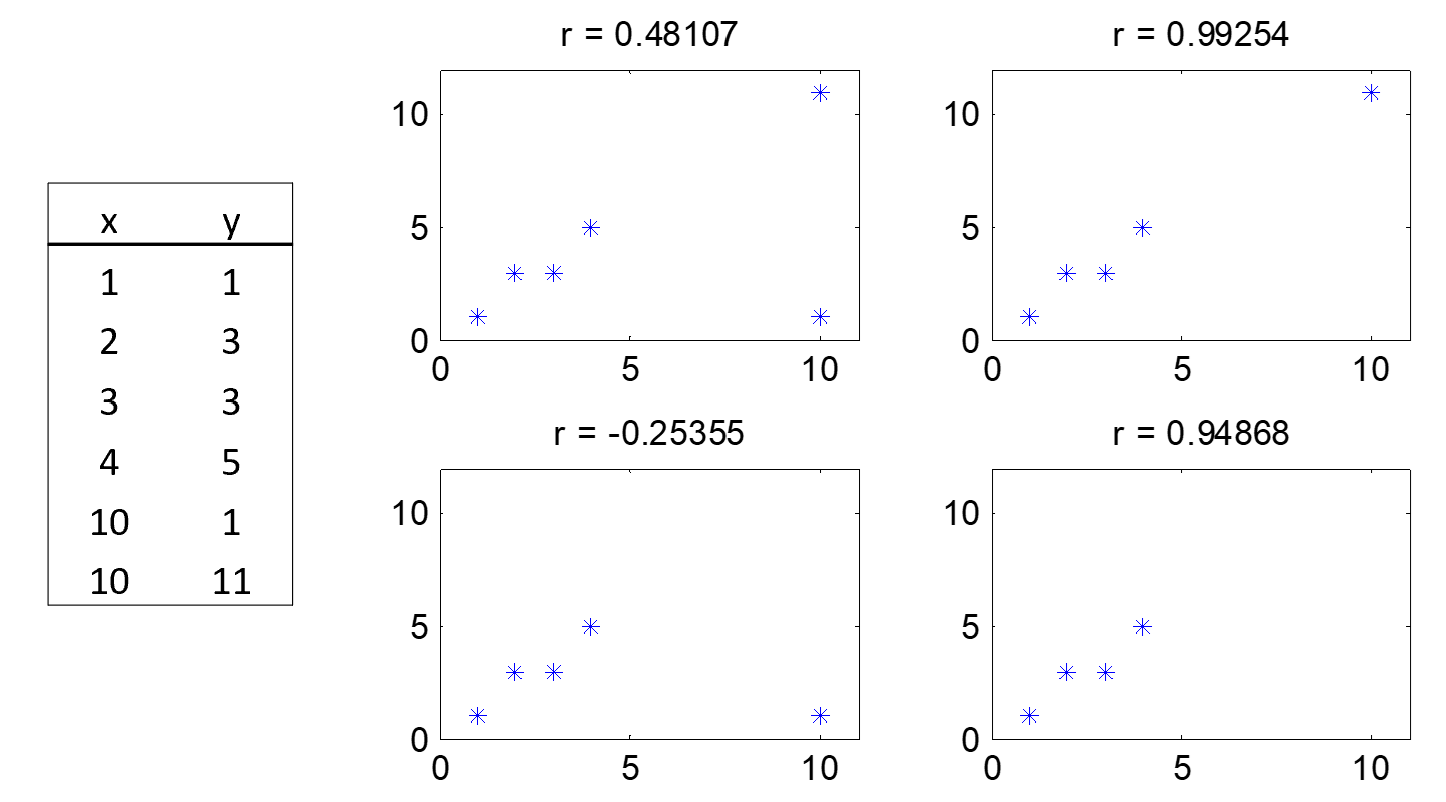
\includegraphics[scale=0.7]{images/outliers.png}
\end{center}

Correlation does not describe nonlinear associations!

\begin{center}
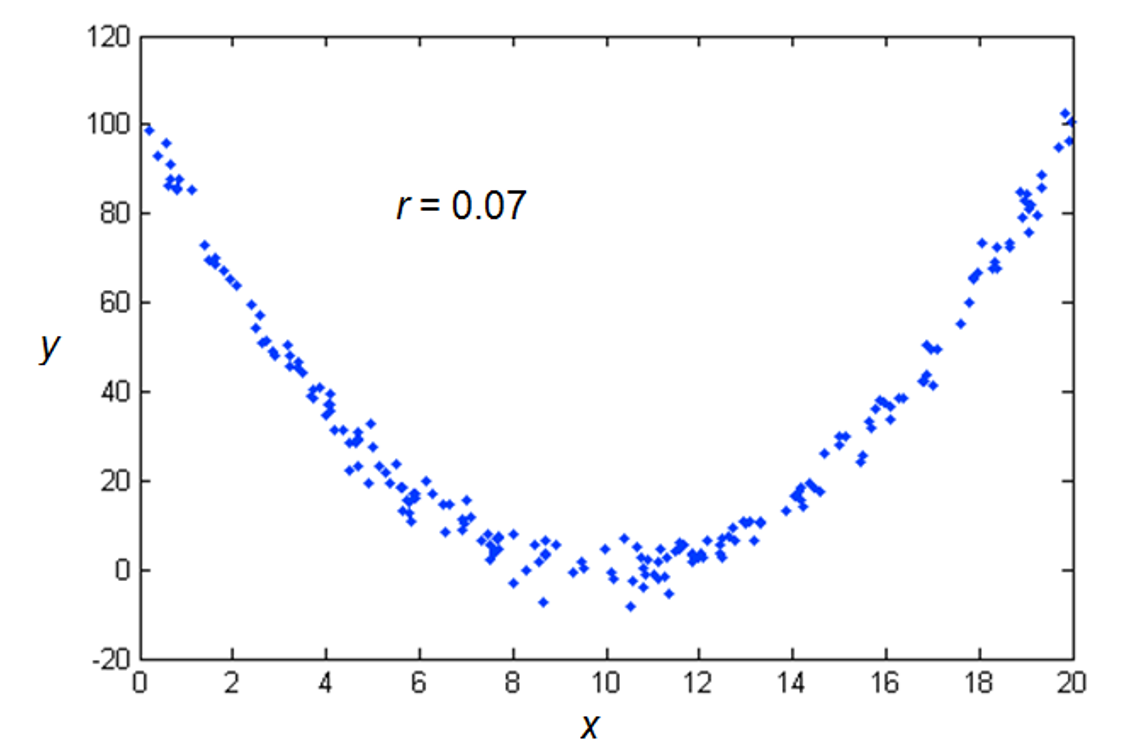
\includegraphics[scale=0.6]{images/nonlinear.png}
\end{center}

\newpage

Practice: Which scatterplot has the largest correlation (closest to +1)?

\begin{center}
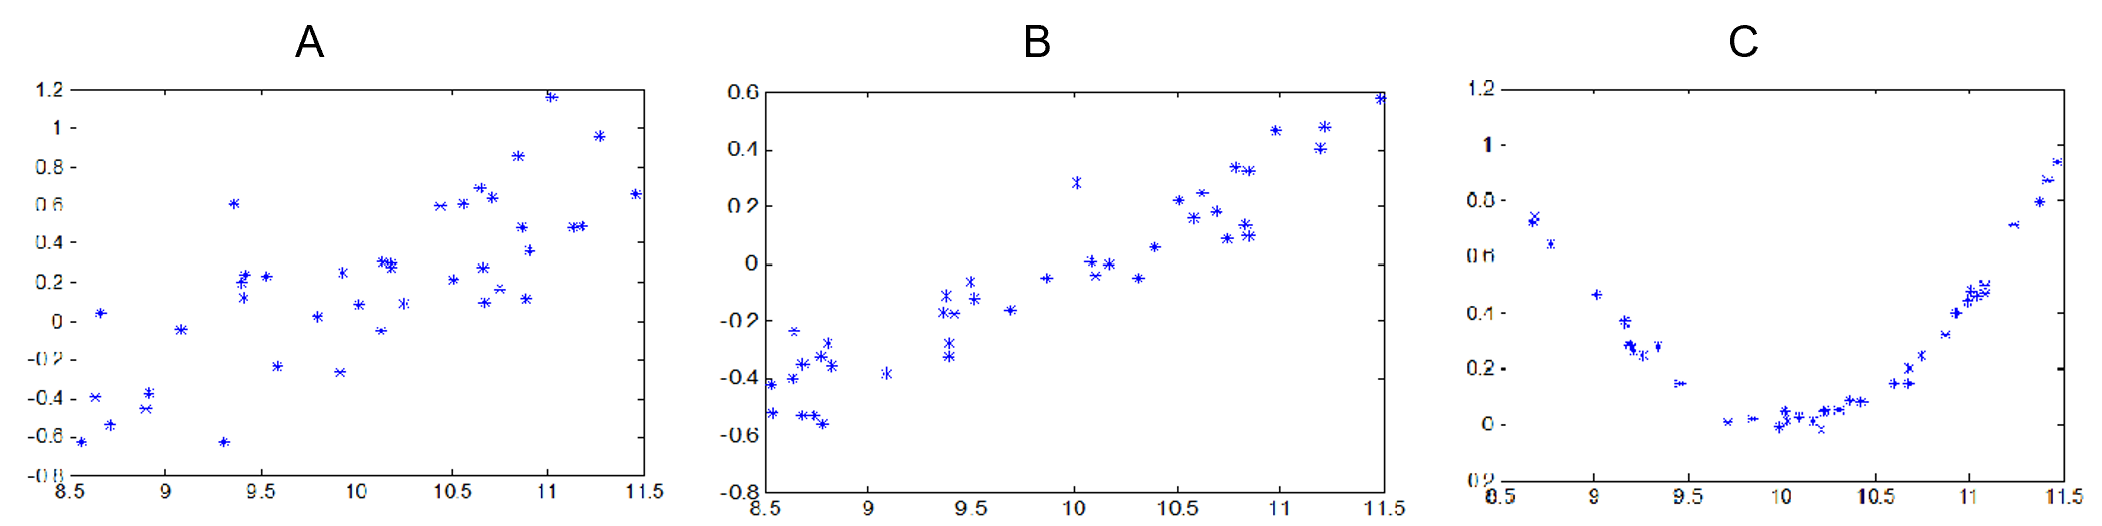
\includegraphics[scale=0.55]{images/practice.png}
\end{center}

Exercise: Heights of couples

The Excel sheet {\tt heights.xlsx} contains the heights of 6 heterosexual couples.

\begin{enumerate}

\item Make a scatter plot and guess at the value of $r$. \vspace{60pt}

\item Calculate $r$ in Excel. \vspace{60pt}

\item If all the men were 6 inches shorter, would correlation change?  Does the correlation tell us about whether women tend to date men taller than themselves? \vspace{60pt}

\item If heights were in centimeters, would correlation change? \vspace{60pt}

\item If each woman dated a man exactly 3 in.\ taller than herself, what would be the correlation?

\end{enumerate}




\label{totalpag}
\end{document}